We will in this chapter discuss poloidal flows in short.
Sheared poloidal flows as they

The term "zonal flow" is used in metrology to describe atmospheric and oceanic circulation along latitudinal lines, such as those observed in Jupiter \cite{Limaye1986}.
In plasma physics, it is common in literature to designate the zonal flow as a background poloidal flow, i.e. the zeroth mode of the poloidal velocity spectrum, generated from the turbulence.
The study of zonal flows has gained a lot attention in the recent years as a radially sheared zonal flow due to its supression of turbulence transport \cite{Diamond2005a}.
There is therefore a predator-prey relationship between the turbulence and the zonal flow.
The turbulence drives a zonal flow which supresses the turbulence.
When the turbulence is supressed the zonal flow is not fed, so it dies out.
This means that the turbuelence grows up, and the story repeats itself.

We note that with the plasma physics definition of a zonal flow, not all poloidal flows are zonal flows.
For example is the sustained poloidal flow at the edge of tokamak plasmas found in the high-confinement mode

Different from the metrological description, not all poloidal flows  a zonal flow
it is common to separate between zonal flow

It is common in the literature to separate between


Very briefly no zonal flows are found as done in Burin, Tynan etc.
The idea is just to communicating this, without using too much time on this chapter.

If included: Briefly zonal flows comes from Reynold stresses, Diamond and Kim paper shows acceleration of zonal flow comes from radial derivative $\expt{\wt{v}_\theta\wt{v}_r}$ as long as a $\partial_t \grad_\perp^2 \phi$ is present in the system.
%
\begin{figure}[htbp]
    \centering
    \begin{subfigure}[h]{0.45\textwidth}
        \centering
        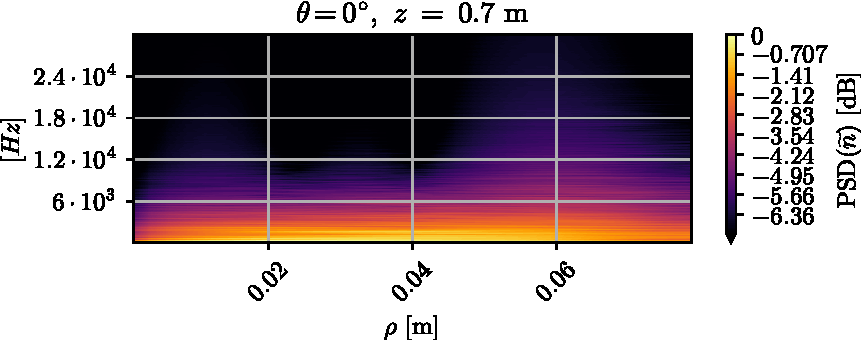
\includegraphics[width=1.0\textwidth]{fig/results/poloidalFlow/PSD2D006}
        \label{fig:PSD2D006}
        \caption{$B=0.06\T$}
    \end{subfigure}%
    \hfill
    \begin{subfigure}[h]{0.45\textwidth}
        \centering
        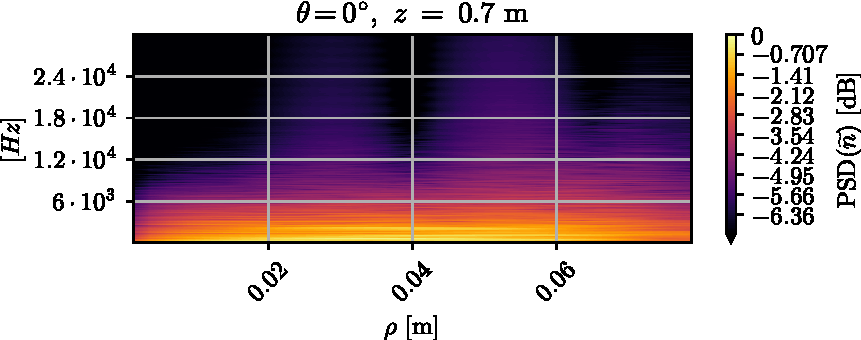
\includegraphics[width=1.0\textwidth]{fig/results/poloidalFlow/PSD2D008}
        \label{fig:PSD2D008}
        \caption{$B=0.08\T$}
    \end{subfigure}
    \\
    \begin{subfigure}[h]{0.45\textwidth}
        \centering
        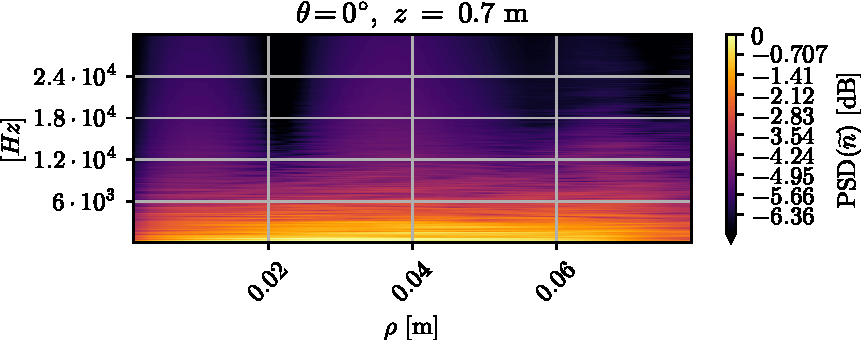
\includegraphics[width=1.0\textwidth]{fig/results/poloidalFlow/PSD2D01}
        \label{fig:PSD2D008B}
        \caption{$B=0.01\T$}
    \end{subfigure}
    \caption{Radial dependency on the power spectral density.}
    \label{fig:PSD2D}
\end{figure}
%
It can be observed in \cref{fig:PSD2D} that the spectra broadens for increasing $B$, and that the main part of the broadening happens outside the maximum of the absolute gradient of $n$.
As stated in ...
the spectra is more narrow when using the Boussinesq approximation.
However, no sustained zonal flow is found from the spectra.
If that was the case, the spectra would be narrowed in the region after the zonal flow as the flow would shear the eddies.
This can also be observed in \cref{fig:zonalFlow0008} which shows a shear only at the very edge of the plasma.
%
\begin{figure}[htb]
    \centering
    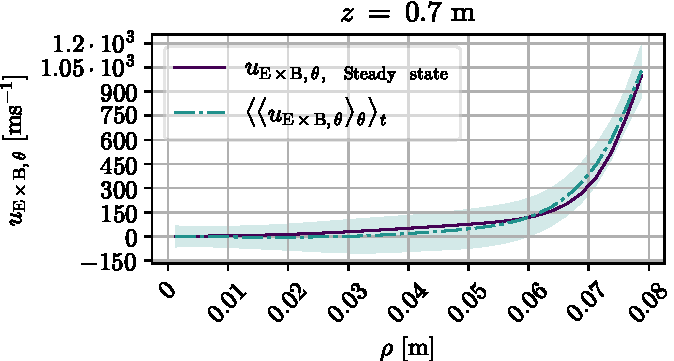
\includegraphics{fig/results/poloidalFlow/poloidalFlow01}
    \caption{Poloidal velocity in the system for $B=0.01\T$}
    \label{fig:zonalFlow0008}
\end{figure}
%
